The frontend is built using the JavaScript framework Angular 4. When deciding what to use the group members decided that it should not only be a good choice for this project but also useful if they would work as frontend developers in the future. This meant that the two most popular modern frameworks React and Angular were suitable alternatives. The smaller and easier to learn Vue was also a contender that provides a lot of the same tools that React and Angular does. All of these use components to build the web application which made it easier to split the work among the group members. The group also wanted a framework that provided good structure to help the developers that had limited experience developing an application of this size.

Both Angular and React have steep learning curves but Angular provides more guidance and a lot of packages are included\cite{jensneuhaus}. In React what packages to use is up to the developers and that was not something the group wanted to spend time on in this project. That is also one of the reasons why Angular is better suited for larger groups since everyone in the project will build the site in a similar way. Angular also provides two-way data binding which means that the model will be updated when the view changes and vice versa\cite{jensneuhaus}. Even though it has some drawbacks it was seen as a great help when developing the site.

Vue has been rising in popularity lately and it was an interesting alternative since it is simpler than both Angular and React. The drawback is that it does not have as much support as the other two who are backed by Google (Angular) and Facebook (React). That means that there are less tutorials for Vue and it is harder to find information about how to solve problems\cite{clockwise}. So even though it might be easier to learn it may take more time to develop things that already has solutions in other frameworks. Therefore the group decided to use Angular but both React and Vue would probably have worked fine for the project as well.

The site consists of the 17 distinct components listed in table~\ref{tab:components}, these make up the different pages as well as various element on the pages that are complex enough to be regarded as separate entities. By dividing the design into smaller parts, both modularity and readability is improved; In the case of the gamification elemente, that modularity is essential and allows teachers to only use what gamification elements they like. And in the case of the user page as well as the course page, it allows heavy reuse of components, which keeps the code concise.

To reduce the amount of time spent with developing a style for the site, the Bootstrap CSS framework was used. Since it provides well-established themes for all HTML elements, a clean and consistent design could be designed early on to serve as a basis for design decisions. On top of that, a color scheme lightly influenced by the LTU webpage was designed to give the site a distinct and personal profile that would also look familiar to the target audience.

\begin{figure}[hb]
    \captionof{table}{All components featured on the site.}
    \centering
    \begin{tabular}{r|l}
        Component Name & Description\\\toprule
Assignment & Assignment submission page\\
Assignment-Group & Assignment group subcomponent\\
Course-Statistics & Per-course statistics page\\
Courses & Detailed course view\\
Create-Assignment & Assignment creation/modification page\\
Create-Course & Course creation/modification page\\
Game Element & Modular game element base-class\\
Head & Sidebar, page header\\
%Join-Course
Login-Helper & Login redirection landing page\\
Login & Pre-login frontpage\\
%Main
Mod-Adventuremap & Modular adventure map subcomponent\\
Mod-Badges & Modular badge subcomponent\\
Mod-Leaderboard & Modular leaderboard subcomponent\\
Mod-Progressbar & Modular progressbar subcomponent\\
Teacher-Courses & Teacher view for courses\\
User-Panels & Element container\\
User & Post-login frontpage, course overview\\\bottomrule

    \end{tabular}
    \label{tab:components}
\end{figure}

\subsection{Login}
To authenticate yourself on login you are by default prompted to sign in with LTU's weblogon CAS (Central Authentication Service). 
This provides you with a ticket as an URL parameter and redirects you to path: \url{https://frontend\_ip/Auth} which in turn contacts backend with said ticket to check its validity. If validated the backend responds with a status code of \texttt{200:\@ OK} and a JSON object containing authentication tokens for the user which are saved in local storage. In any other case the user receives status code \texttt{401:\@ Unauthorized} and is prompted to login again.
\begin{figure}[H]
    \centering
    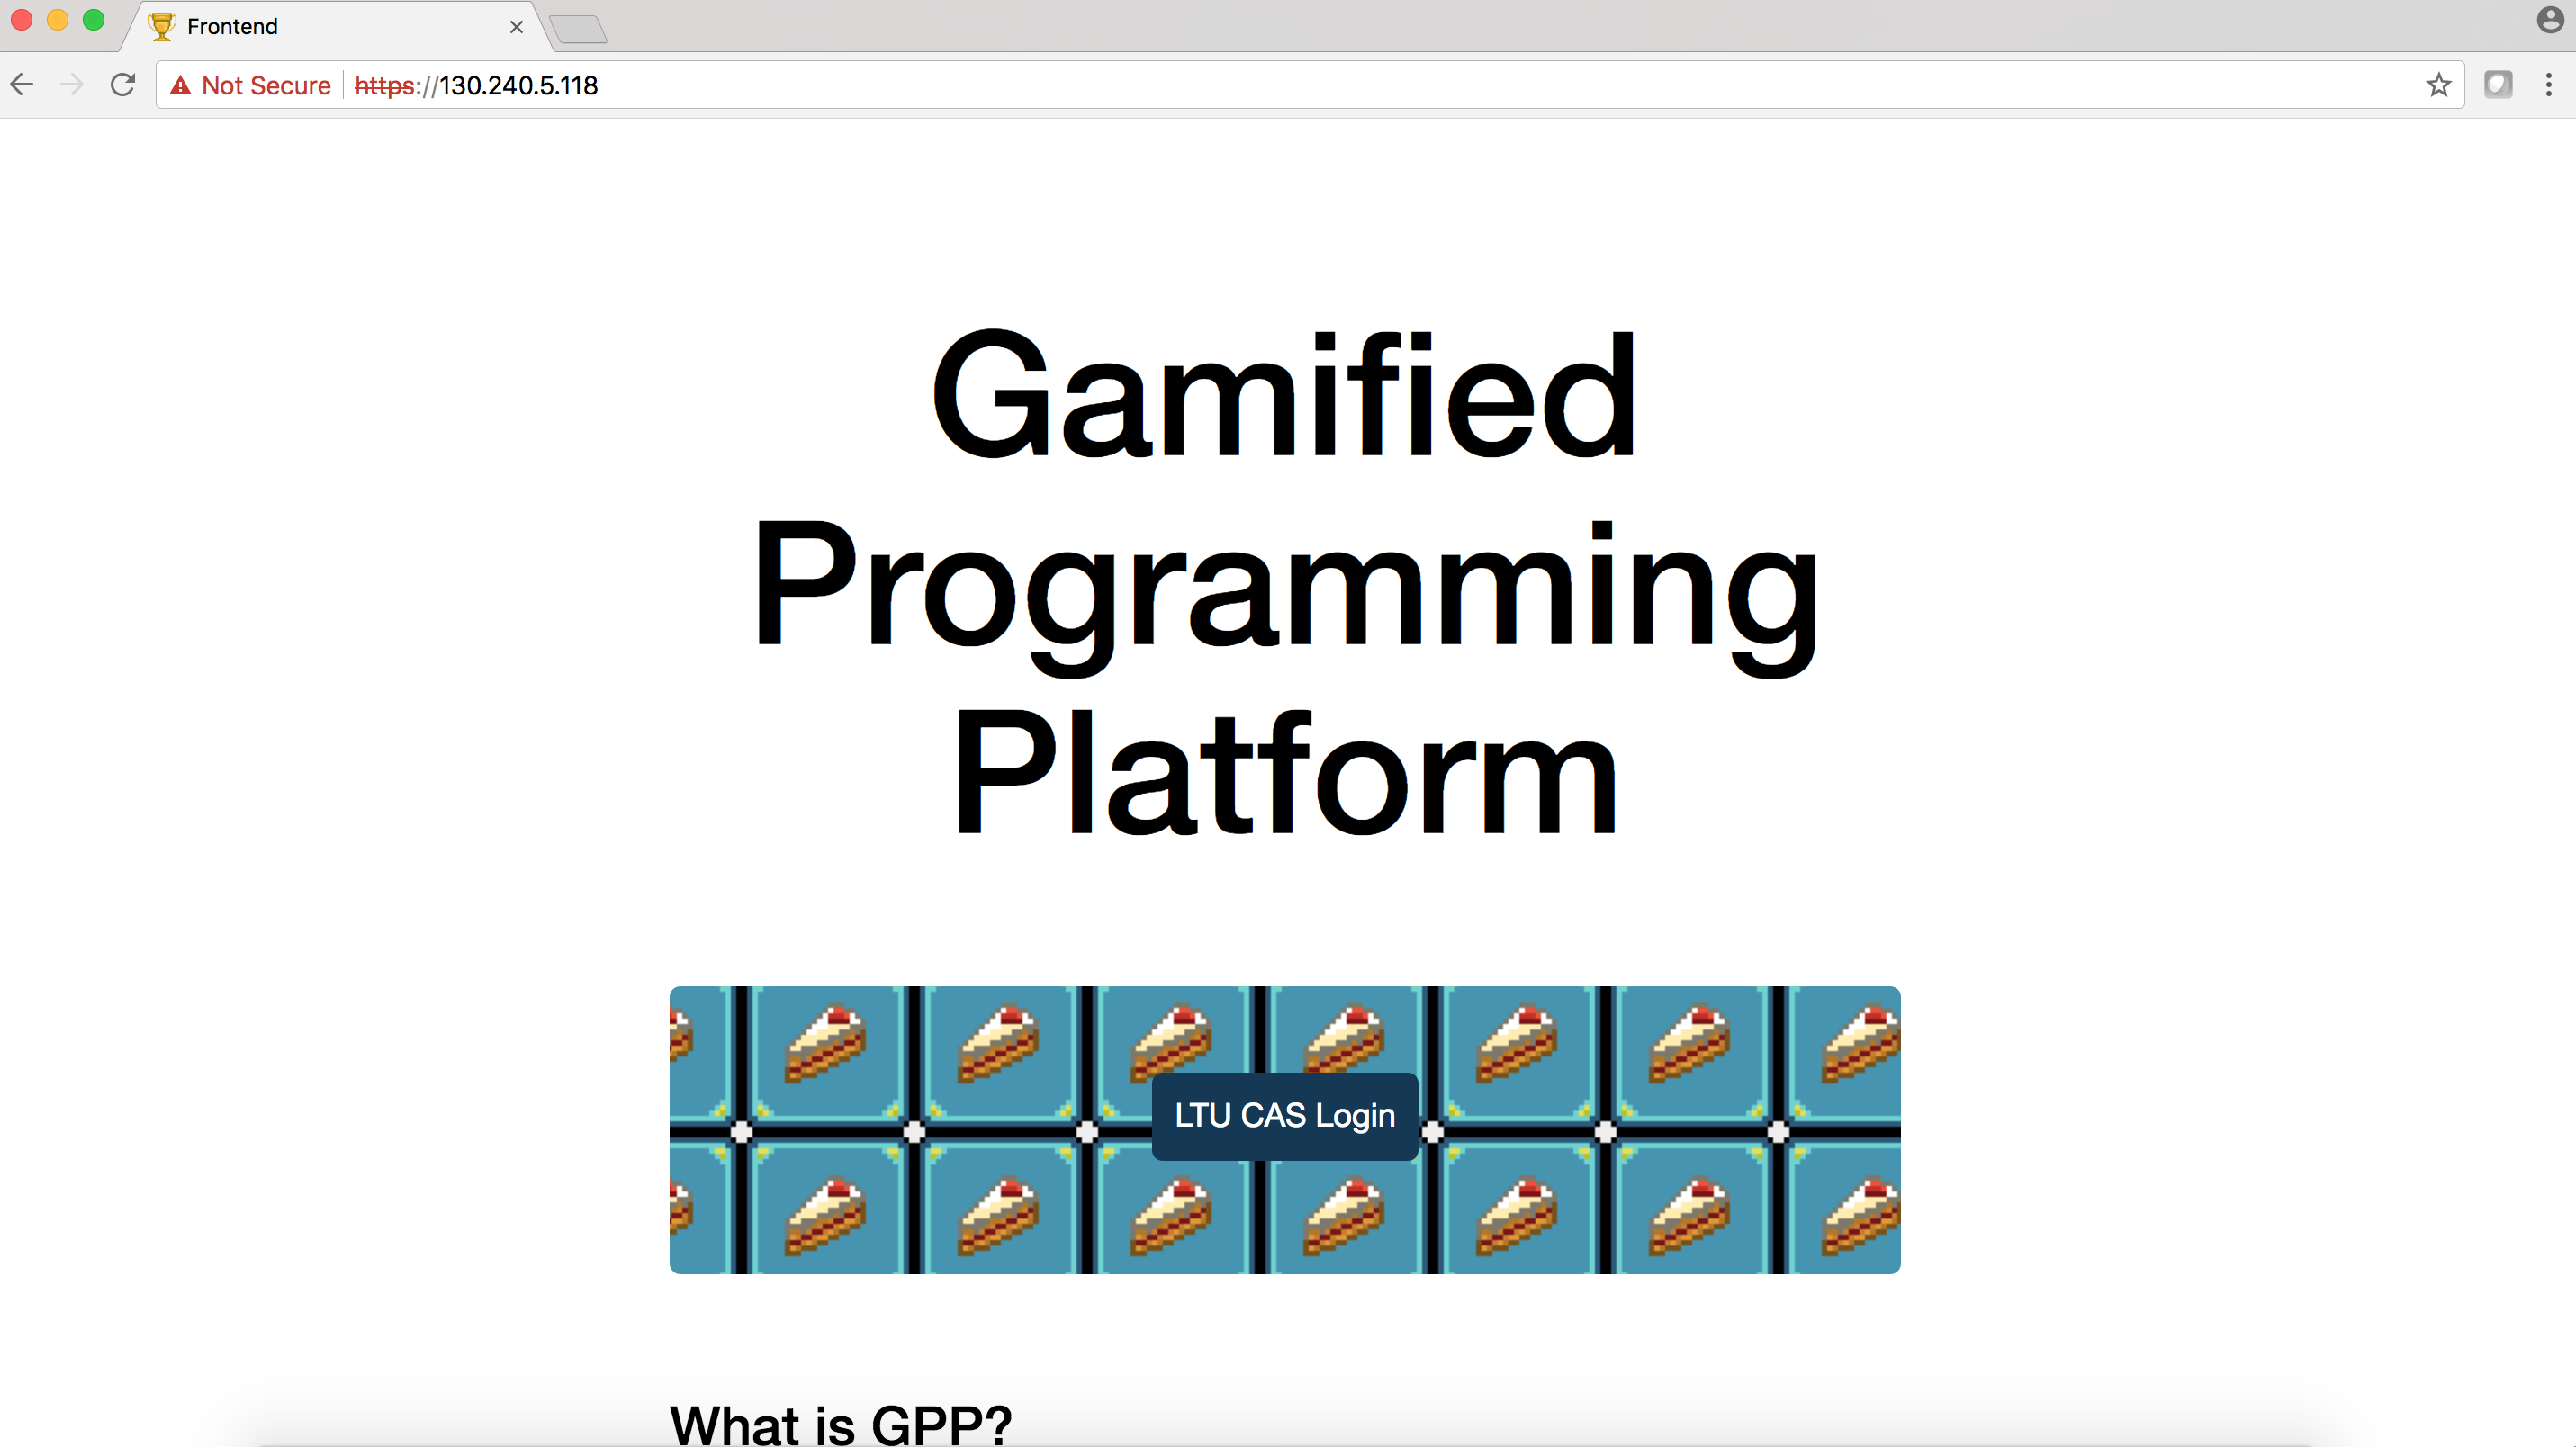
\includegraphics[width=.45\textwidth]{img/gppinpictures/login2.png}
    \caption{A screenshot depicting the landing page for a user.}
    \label{fig:student}
\end{figure}

\subsection{User Page}
Since the user page acts as the front page of the site it should display a good overview to the user. Therefore all courses that a user either has joined or created will be displayed here. To not take up too much space each course is a collapsed panel that can be opened to show any gamification elements available in the course. By clicking on the name of the course the user will be redirected to the page for that course.

It is also possible to join a course by selecting a course from a list. This list is displayed in a modal opened by the button above the courses you have joined.  The list does not only show the course code or the name of the course but also the creator of the course. This is because there can be many courses with the same name and/or code.

On the right half of the page you can see which courses you have sent join-requests to and what requests have been sent to your courses. The courses that have allowed students to join the course directly without any confirmation from the teacher will of course not be displayed here. Below the requests there's a list showing any invites sent by teachers to the user. The invites can be accepted or declined.
\begin{figure}[H]
    \centering
    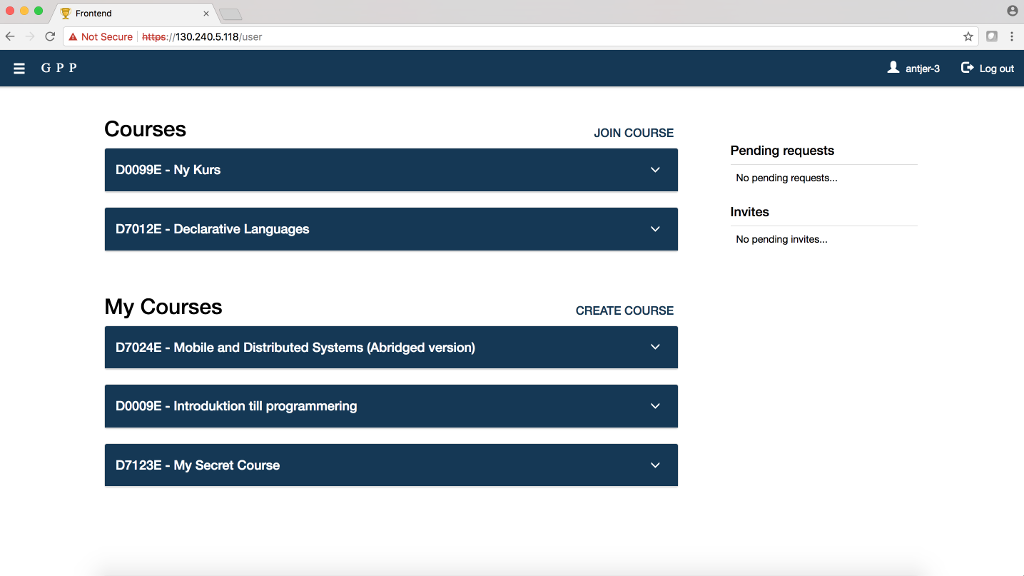
\includegraphics[width=.5\textwidth]{img/gppinpictures/user.png}
    \label{fig:student}
    \caption{The front-page view for a user}
\end{figure}

\subsection{Course}
A user can be a student or a teacher in a course, therefore it felt natural to have two different course pages with corresponding functionality. That is, the student view shows the progress of a single user and the teacher view shows the progress of all students. A user can also create courses which it will be a teacher of. 

\subsubsection{Student Course Page}
The student course page can be viewed by students that are registered on a course. To have a good overview, panels similar to the user page are used to display different gamification elements that may be available to the course along with the assignments, which is sorted by groups. The assignments are displayed in collapsible panel groups that allow the students to view the assignments and groups in an efficient way. If an assignment is clicked, the student will be directed to the assignment page. 

% I might have described the gamification elements a bit too much here?
Depending on which gamification elements are enabled for the course, students will have different layouts. If for example the adventure map module is enabled, a student can see its progress on the map, if it is disabled, the student will not see it.

For instance, say all gamification elements are available, then the student would first see a progress bar. This displays how many assignments the student has completed of a total amount. Then, the student would see the badges, this shows all badges a student has managed to collect, depending on which test and assignments have been passed. After that comes the leader board, which simply displays the score for each student in sorted order. Finally the adventure map, it presents groups and assignments together with a narrative, so the student can see its advancement and what is left and read a story that goes along with the progress.
\begin{figure}[H]
    \begin{subfigure}{.48\linewidth}
        \centering
        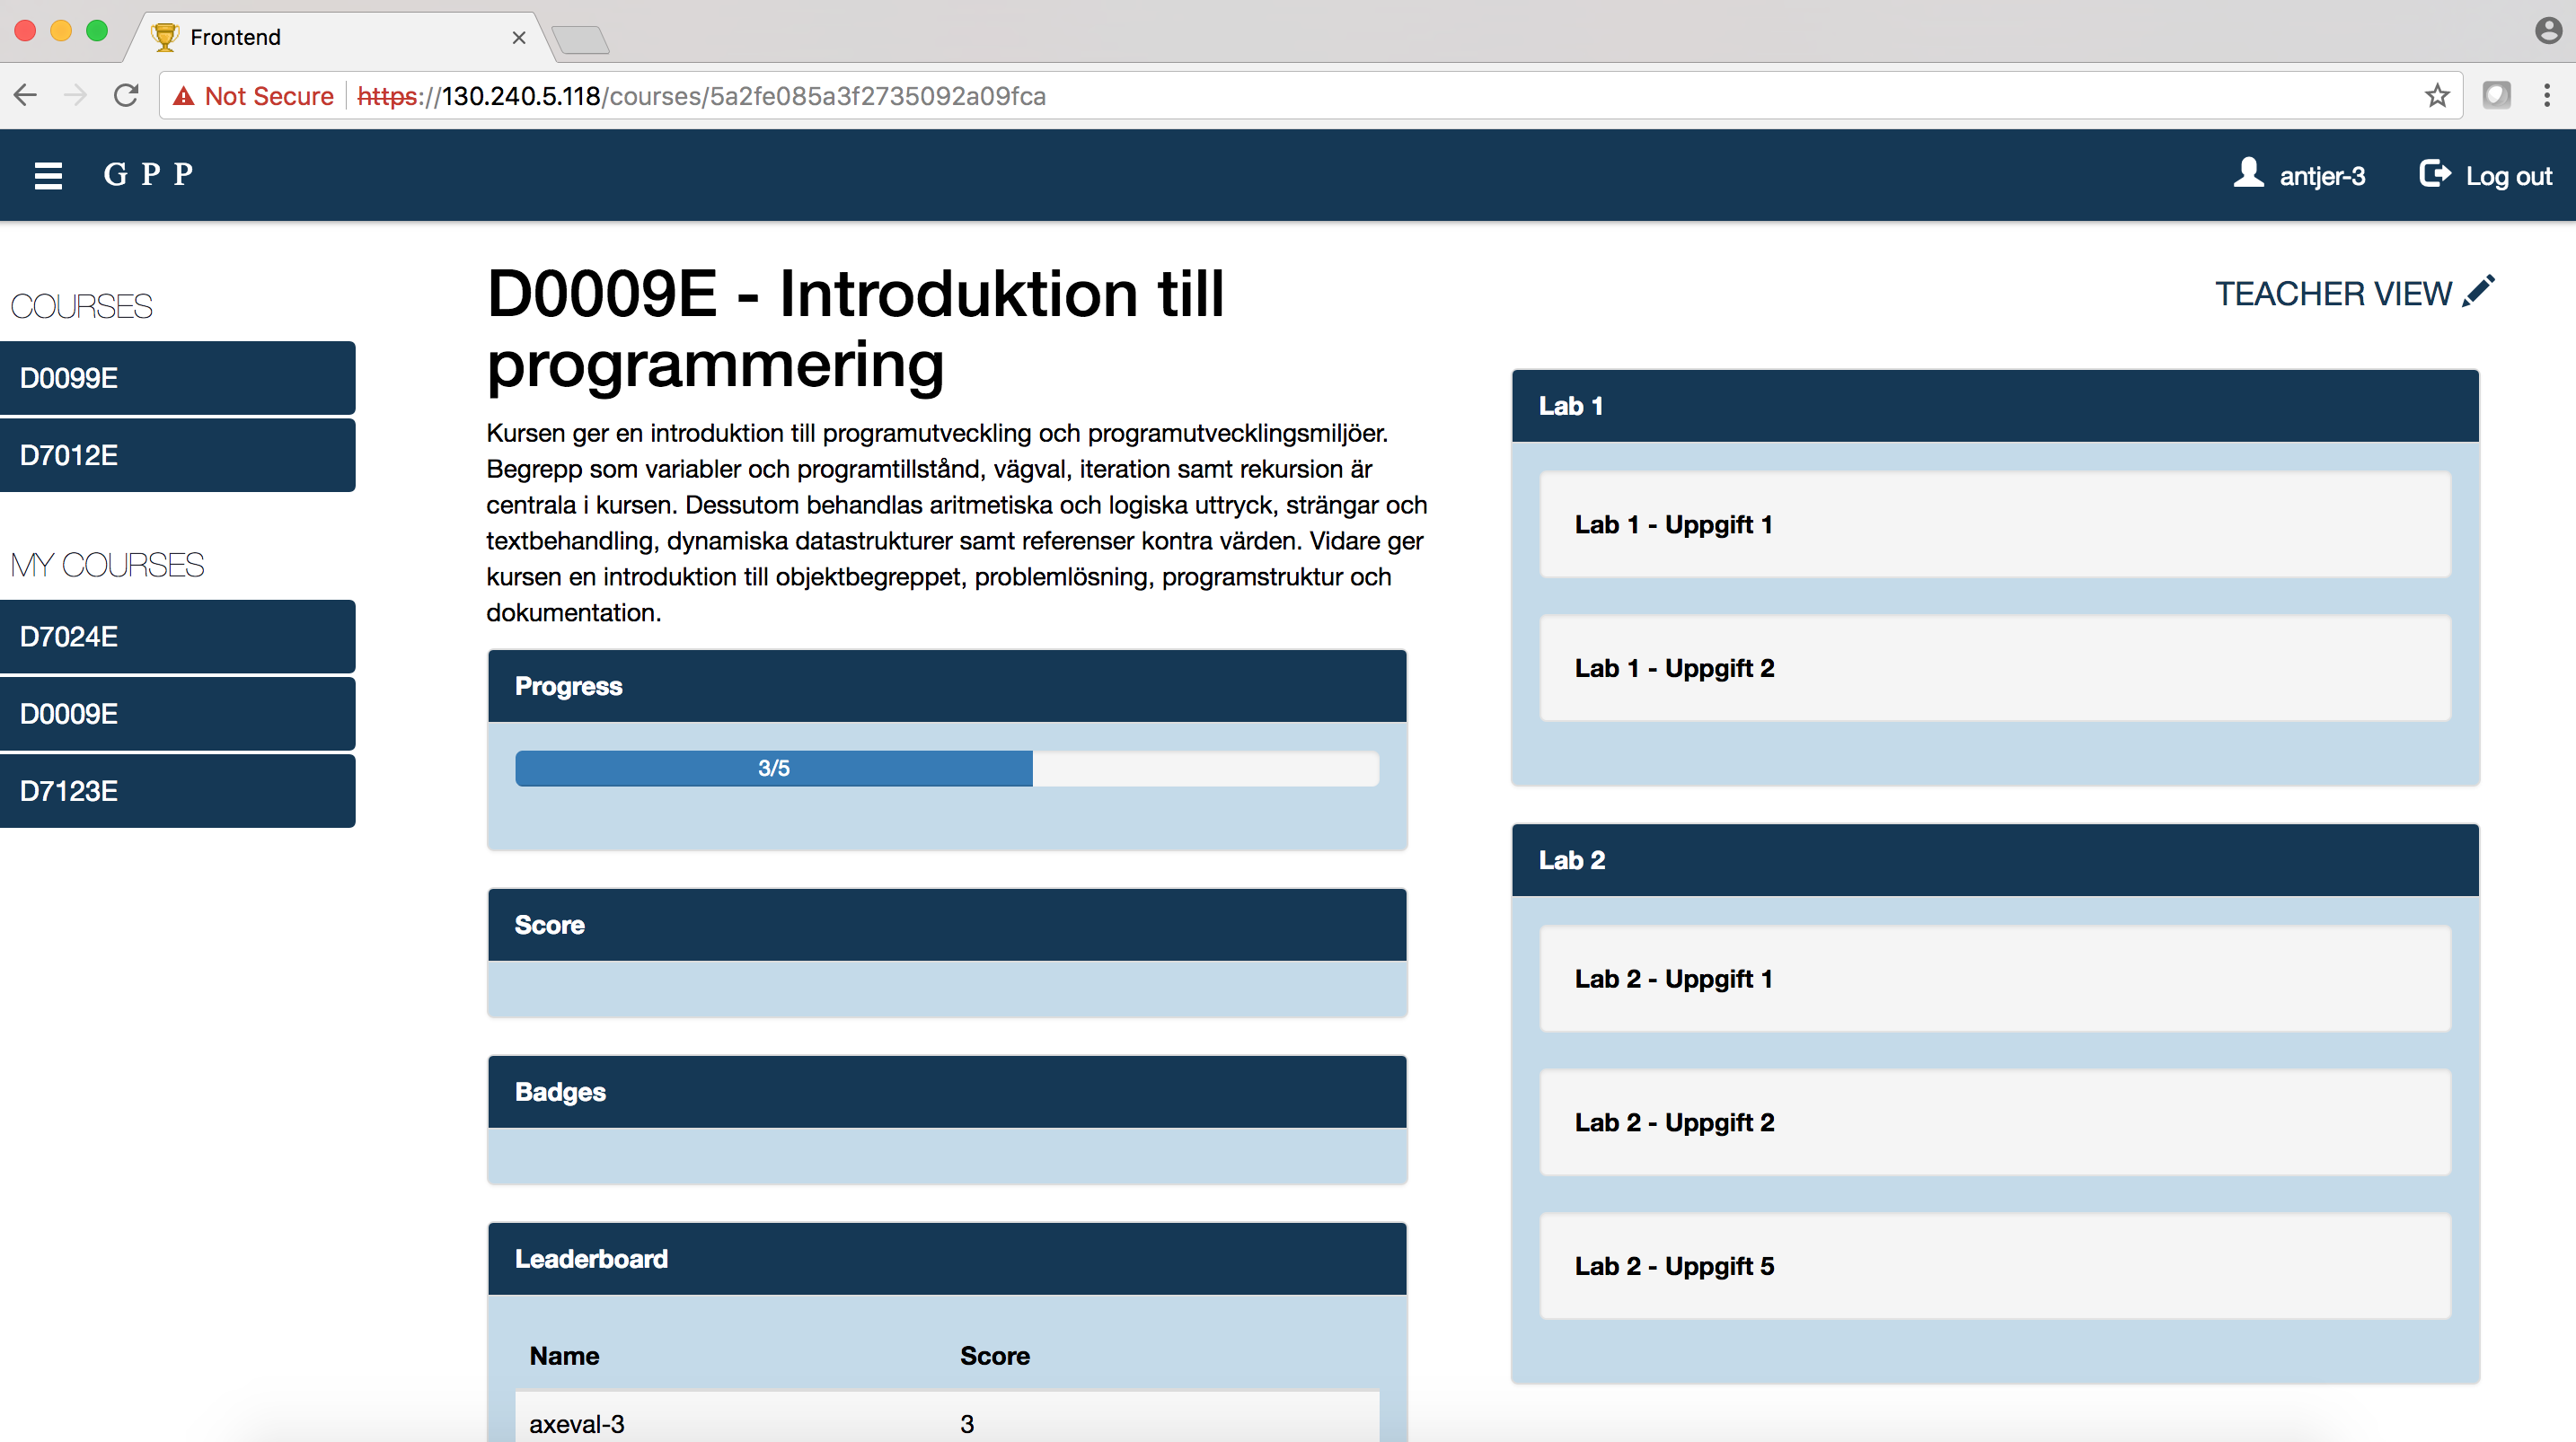
\includegraphics[width=\textwidth]{img/gppinpictures/studentview.png}
        \caption{Student view for a course}
        \label{fig:student}
    \end{subfigure}
    \hfill
    \begin{subfigure}{.48\linewidth}
        \centering
        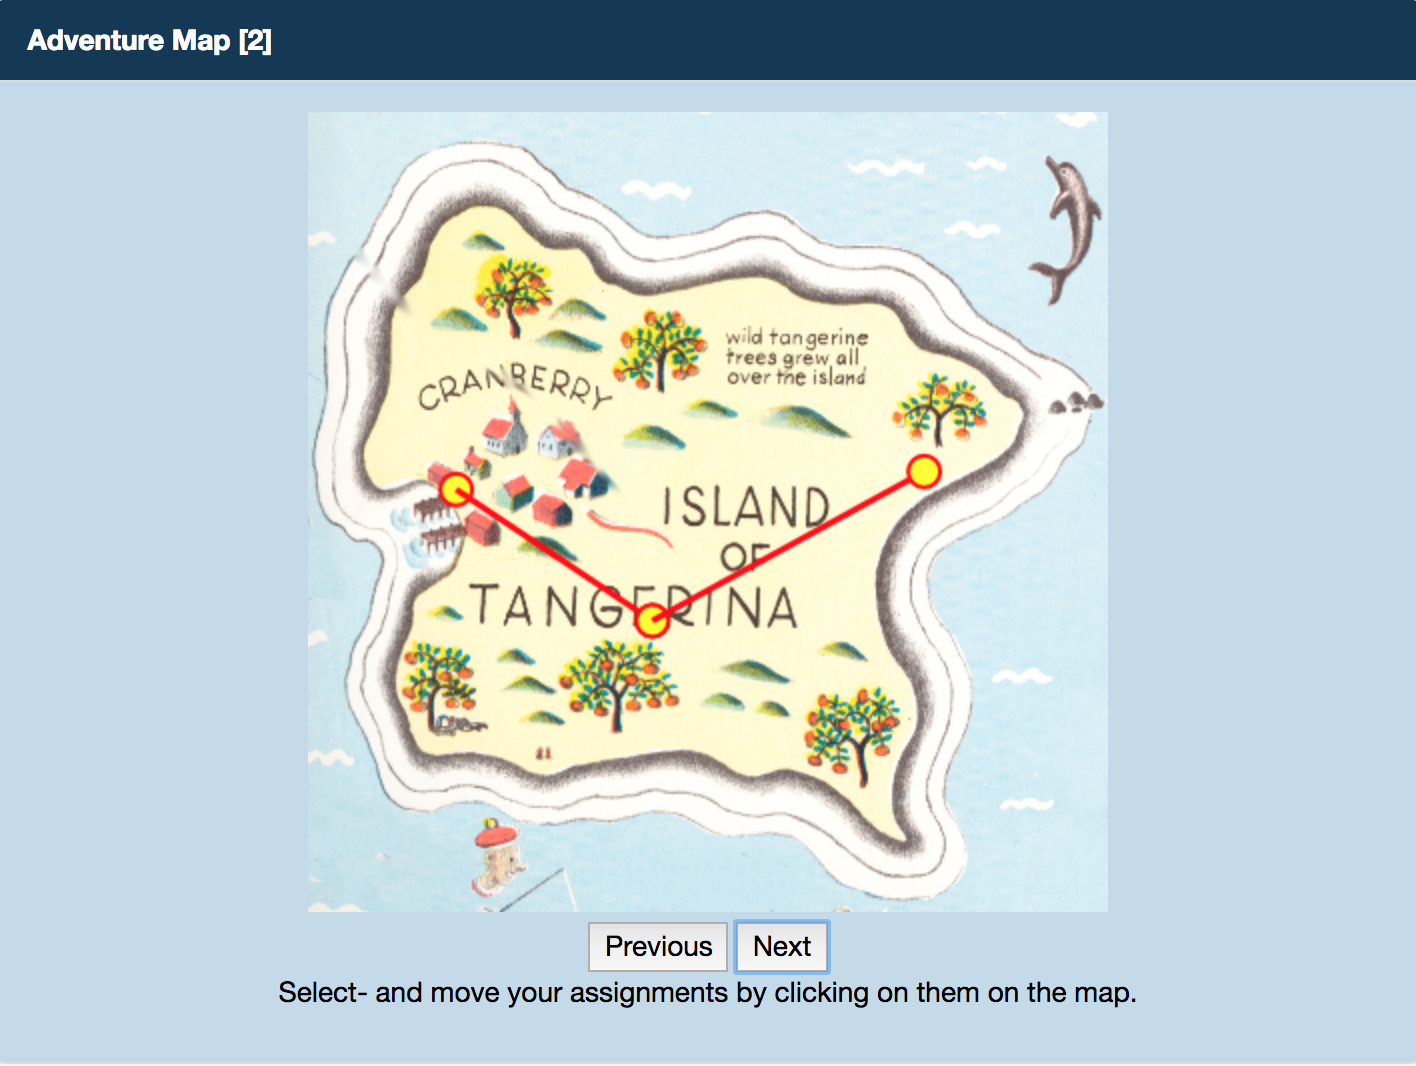
\includegraphics[width=\textwidth]{img/gppinpictures/adventuremap.png}
        \caption{An adventure map}
        \label{fig:student}
    \end{subfigure}
    \caption{Two ways of representing a course.}
\end{figure}

\subsubsection{Teacher Course Page}
The teacher page has a bit more functionality than the student page. It is here teachers can view and modify their courses and create groups, badges or manage adventure map. A teacher can see the course's description and click on edit to update the course. Under the title ``Assignments'' the teacher can view all assignments for the course, or create a new one. It is also possible for the teacher to create groups by a simple button click. Adding assignment to a group is done using an intuitive drag and drop method. 

If the adventure map is available for the course there is the possibility for the teacher to arrange assignments by groups and place them out on the map. If badges are an enabled feature a teacher can create a new badge, associate it with assignments and tests that is necessary for a student to pass before it can receive the badge.

For a comprehensive layout all student related information are put in a column on the right side. Here the teacher can see requests from students, invitations the teacher have sent to students and also students that are enrolled to the course. There is also options for the teacher to accept or decline a request from students, delete an invitation and add a student to the course. 

Adding a student to a course can be done in several ways. A teacher can either search for a student using its username and then send an invitation, or the teacher can generate an invitation link. The invitation link can be sent out to students who can then use it to join a course directly. It is also possible for the teacher to view invitations links, to see its code, how many times it has been used and when it expires. There is also the possibility to cancel the link.

The teacher can also toggle between student and teacher view. The teacher can use this to go through their own courses with groups and assignments to control so that everything is in order. 

\subsubsection{Create Course}
Creating a course is possible for both ordinary students and teachers. However, students are only allowed to create a maximum of three courses whereas teachers can create any amount. The create course component is also used for updating a course. A course consists of a name, course code, description and the optionally enabled features. Whether the course should be public and if it should be auto-joinable is visualized as check boxes.

Enabled features are made up of a progress bar, badges, the adventure map and the leader board, this decides if a gamification element should be available in the course or not. Public means that the teacher will make the course public so students can see, request access or join the course. Auto join means that students will be able to join the course freely so no request is required. The course description uses markdown, same as the create assignment page. 

When a course is submitted, an API call to backend to create a new course will be made. If it was successful, the response will be used in the course service to add the new course to the database. By using subscriptions, all concerned components will be notified and updated in real-time.
\begin{figure}[H]
    \centering
    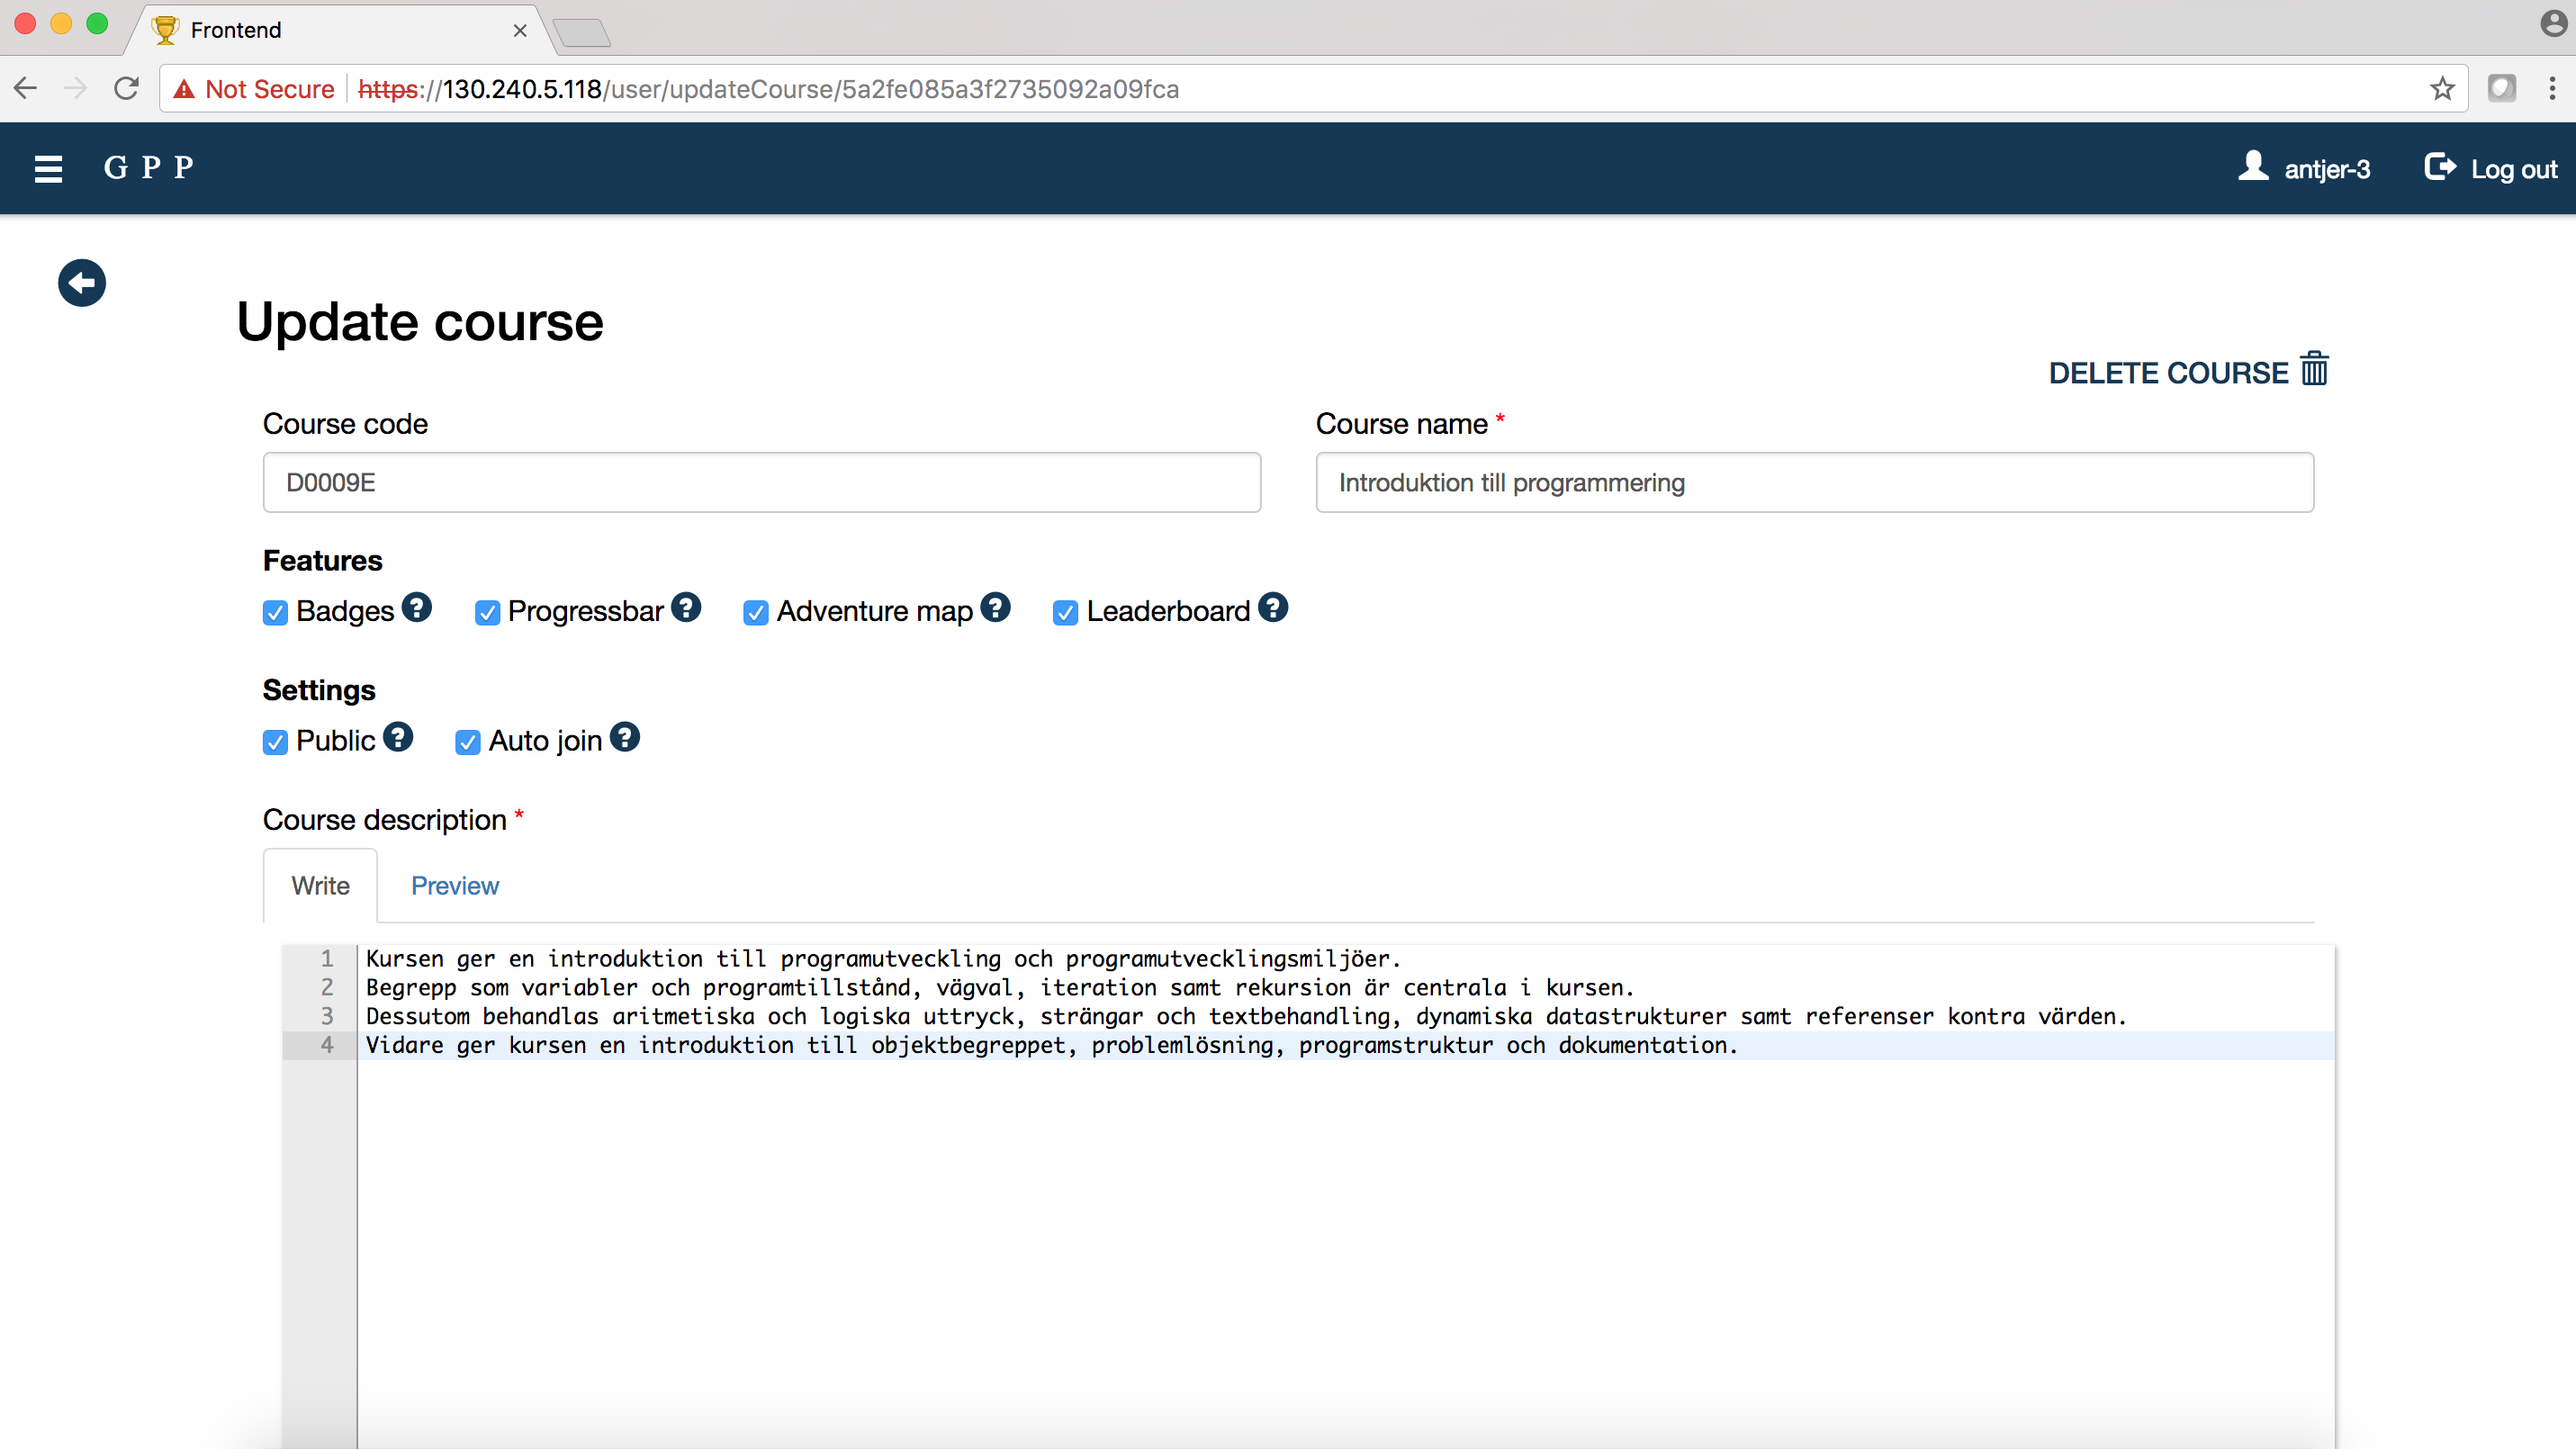
\includegraphics[width=.5\textwidth]{img/gppinpictures/editcourse.png}
    \caption{The course creation page.}
\end{figure}

\subsection{Assignment}
\subsubsection{Assignment Page}
The assignment component is used for displaying and for submitting a solution to an assignment. The component consists of three key fields. A feedback field for displaying server response from tester. A description field for showing the assignment description and finally an in-browser editor. 

The decision to implement an in-browser editor for writing the code was made early on as it was seen as more intuitive than having to write your code using your own editor and then uploading files to the site.

CodeMirror was used to implement the first iteration, however, this editor was dropped and replaced by an implementation of ace editor, which had far many more options in terms of customization such as size of editor and theme. Ace editor also had better support for switching between syntax highlighting of different languages, while CodeMirror required us to reload editor upon switching language. 
\begin{figure}[H]
    \centering
    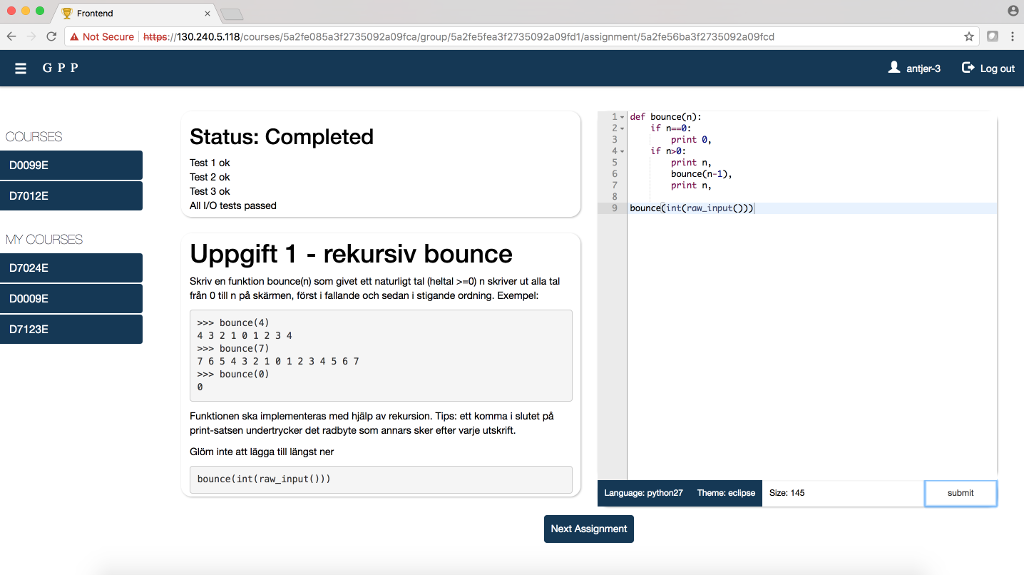
\includegraphics[width=.5\textwidth]{img/gppinpictures/assignment.png}
    \caption{The assignment submission page.}
\end{figure}

\subsubsection{Create Assignment}
The create assignment page is used for both creating and editing assignments. An assignment consists of a name, description, available languages and flag whether or not the syntax of the code should be tested using lint. 

By implementing markdown---a markup language for HTML---teachers are able to add different sized headers, lists, embedded pictures, links and code blocks with syntax highlighting. Early versions of the create assignment page implemented a live-preview for writing the description, however it got removed to maintain consistent design with the create course page. 

In addition to this, the create assignment page contains a field for creating and editing input-output tests. A teacher can add multiple tests for verifying the code against multiple inputs.

Once an assignment is ready to be submitted, an API call to backend to create new assignment will be made and if that call is successful, additional calls for adding input-output tests can be made. 
\begin{figure}[hb]
    \centering
    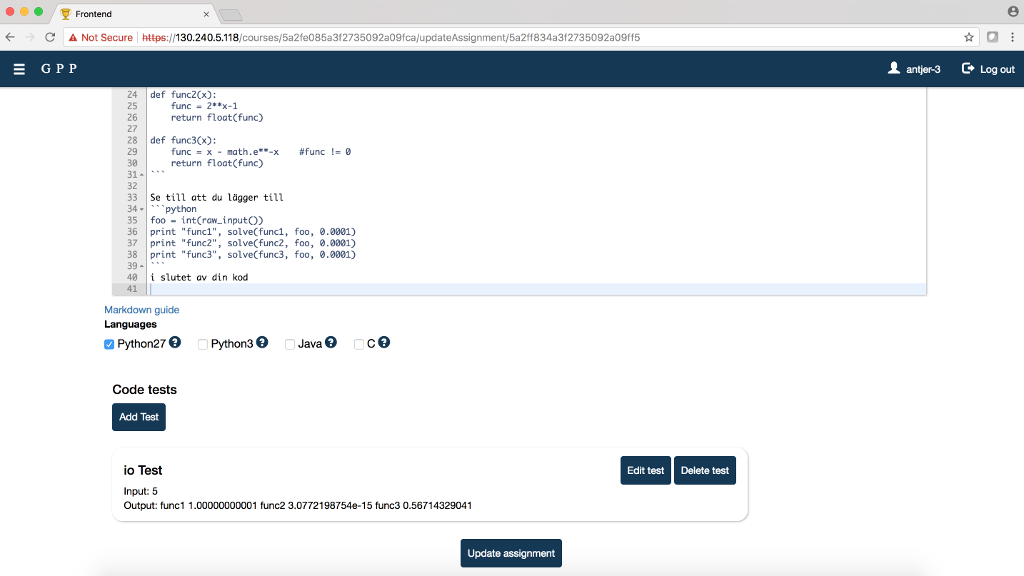
\includegraphics[width=.5\linewidth]{img/gppinpictures/editassignmenttests.png}
    \caption{Edit assignment}
\end{figure}

\subsection{Services}
In Angular, a service is a function or object that is accessible from anywhere in the application. On the frontend, services are used regularly as a means to reuse code, such as API calls to backend, as well as to maintain data across several pages. In the following sections some of the more important and well-used services are detailed.

\subsubsection{BackendService}
The BackendService is the center of all our communication with the backend. Every component or service that needs to either get or post information to or from the backend does so through this service. By requiring all calls to go through this service, all error handling can be made in one place and ensure that all calls are sent in a similar fashion. All calls expects a response with a JSON body, if there is no relevant information to send in the body an empty JSON body should be sent.

All of functions in the BackendService return a Promise that will eventually resolve to the response from the backend. In the event that a request fails, a Toast containing the error message is displayed to the user. 

\subsubsection{AssignmentService and CourseService}
The AssignmentService is used to keep track of assignments belonging to a specific course. Information about assignments are stored in the service to remove the need of fetching assignments all the time when navigating the course page (e.g., going from the course page to the assignment page and back). The service is also used to keep the information up-to-date with changes that comes as a result of user action. For example, if a teacher creates a new assignment, we only fetch the new assignment from backend and adds it to the already saved list of assignments.

The CourseService fulfil the same purposes as the AssignmentService, but for courses instead of assignments as the name suggests.
